\documentclass[a4paper,]{article}
\usepackage{lmodern}
\usepackage{amssymb,amsmath}
\usepackage{ifxetex,ifluatex}
\usepackage{fixltx2e} % provides \textsubscript
\ifnum 0\ifxetex 1\fi\ifluatex 1\fi=0 % if pdftex
  \usepackage[T1]{fontenc}
  \usepackage[utf8]{inputenc}
\else % if luatex or xelatex
  \ifxetex
    \usepackage{mathspec}
  \else
    \usepackage{fontspec}
  \fi
  \defaultfontfeatures{Ligatures=TeX,Scale=MatchLowercase}
\fi
% use upquote if available, for straight quotes in verbatim environments
\IfFileExists{upquote.sty}{\usepackage{upquote}}{}
% use microtype if available
\IfFileExists{microtype.sty}{%
\usepackage{microtype}
\UseMicrotypeSet[protrusion]{basicmath} % disable protrusion for tt fonts
}{}
\usepackage[margin=1in]{geometry}
\usepackage{hyperref}
\hypersetup{unicode=true,
            pdftitle={Identifying suitable locations for onshore wind turbines using a GIS-MCDA approach},
            pdfauthor={Michael Harper, Ben Anderson, Patrick James, AbuBakr Bahaj},
            pdfborder={0 0 0},
            breaklinks=true}
\urlstyle{same}  % don't use monospace font for urls
\usepackage{longtable,booktabs}
\usepackage{graphicx,grffile}
\makeatletter
\def\maxwidth{\ifdim\Gin@nat@width>\linewidth\linewidth\else\Gin@nat@width\fi}
\def\maxheight{\ifdim\Gin@nat@height>\textheight\textheight\else\Gin@nat@height\fi}
\makeatother
% Scale images if necessary, so that they will not overflow the page
% margins by default, and it is still possible to overwrite the defaults
% using explicit options in \includegraphics[width, height, ...]{}
\setkeys{Gin}{width=\maxwidth,height=\maxheight,keepaspectratio}
\IfFileExists{parskip.sty}{%
\usepackage{parskip}
}{% else
\setlength{\parindent}{0pt}
\setlength{\parskip}{6pt plus 2pt minus 1pt}
}
\setlength{\emergencystretch}{3em}  % prevent overfull lines
\providecommand{\tightlist}{%
  \setlength{\itemsep}{0pt}\setlength{\parskip}{0pt}}
\setcounter{secnumdepth}{5}
% Redefines (sub)paragraphs to behave more like sections
\ifx\paragraph\undefined\else
\let\oldparagraph\paragraph
\renewcommand{\paragraph}[1]{\oldparagraph{#1}\mbox{}}
\fi
\ifx\subparagraph\undefined\else
\let\oldsubparagraph\subparagraph
\renewcommand{\subparagraph}[1]{\oldsubparagraph{#1}\mbox{}}
\fi

%%% Use protect on footnotes to avoid problems with footnotes in titles
\let\rmarkdownfootnote\footnote%
\def\footnote{\protect\rmarkdownfootnote}

%%% Change title format to be more compact
\usepackage{titling}

% Create subtitle command for use in maketitle
\newcommand{\subtitle}[1]{
  \posttitle{
    \begin{center}\large#1\end{center}
    }
}

\setlength{\droptitle}{-2em}
  \title{Identifying suitable locations for onshore wind turbines using a
GIS-MCDA approach}
  \pretitle{\vspace{\droptitle}\centering\huge}
  \posttitle{\par}
  \author{Michael Harper, Ben Anderson, Patrick James, AbuBakr Bahaj}
  \preauthor{\centering\large\emph}
  \postauthor{\par}
  \date{}
  \predate{}\postdate{}

\usepackage{xcolor}
\usepackage{mdframed}
\usepackage{booktabs}
\usepackage{longtable}

\usepackage{amsthm}
\newtheorem{theorem}{Theorem}[section]
\newtheorem{lemma}{Lemma}[section]
\theoremstyle{definition}
\newtheorem{definition}{Definition}[section]
\newtheorem{corollary}{Corollary}[section]
\newtheorem{proposition}{Proposition}[section]
\theoremstyle{definition}
\newtheorem{example}{Example}[section]
\theoremstyle{remark}
\newtheorem*{remark}{Remark}
\begin{document}
\maketitle

% Change font for all document
{\fontfamily{cmss}\selectfont
  \renewcommand{\encodingdefault}{T1}
  \renewcommand{\rmdefault}{cmss}

\begin{mdframed}[backgroundcolor=black!5] 
Paper presented in "Proceedings of SET 2017 - The 17th International Confference on Sustainable Energy Technologies, July 17 - July 20 2017, Bologna, Italy"
\end{mdframed}

\section*{Abstract}\label{abstract}
\addcontentsline{toc}{section}{Abstract}

Onshore wind generation is one of the most cost-effective methods of
renewable electricity generation. However, there is often difficulty in
identifying suitable sites for development. To assist such systems,
geospatial information systems are extensively used in identifying
suitable sites for wind turbines: these models predominantly focus on
the technical and legislative constraints, and have a limited
understanding of the social issues surrounding development. As a result,
there are concerns with the validity of these models in accurately
determining suitable sites and fail to acknowledge the strong local
opposition which some projects can experience. Building upon previous
statistical analysis, this paper presents a geospatial multi-criteria
decision analysis that integrates the technological, legislative, and
social constraints to determine suitable sites for onshore wind turbine
development. To the authors' knowledge, this is the first study that
aims to understand whether suitable sites are likely to receive planning
permission and to integrate this into the decision-making process. The
findings highlight the importance of considering the planning
constraints within modelling and demonstrates the limitations in
identifying suitable sites for development.

\section{Introduction}\label{introduction}

Increased environmental concern and issues surrounding security of
supply have led to a global drive to develop renewable energy systems.
This has led to a large increase in the development of these
technologies, which has resulted in significant interest in identifying
suitable locations for these to be installed.

While onshore wind power generation is now both a mature technology and
competitive with traditional energy supplies in many countries, there
are difficulties in identifying suitable sites for wind turbine farms.
To assist this development, many geospatial models have been proposed.
However, there are concerns that current models provide limited
actionable guidance, and in particular fail to account for the
challenges faced in projects obtaining planning permission. This can be
highlighted in the United Kingdom, where more than 50\% of wind turbine
projects in the United Kingdom are rejected at planning (DECC, 2016),
suggesting that wind turbines are being proposed in areas which are
socially unsuitable for development.

The overall objective of the programme of work, to which this paper
contributes, is to build a predictive model for locating onshore wind
turbine projects, integrating resource availability and the likelihood
of a project receiving planning acceptance. In the first stage,
statistical analysis was conducted to identify the key influences for
planning acceptance of onshore wind turbines. This paper presents the
second stage of the analysis, outlining the geospatial model developed
for assessing site suitability and decision making for identifying
suitable sites for wind turbine development.

The work presented here has four parts: an overview of the literature
relevant to onshore wind GIS modelling; a description of the research
methodology; presentation of the model results and finally discussion of
the theoretical and practical implications of the research and further
research opportunities.

\section{Background}\label{background}

Identifying suitable locations for onshore wind turbines requires the
assessment of a range of largely geospatial parameters. As a result,
there has been extensive use of Geographic Information Systems (GIS)
which are designed to capture, store, manipulate, analyse, manage, and
present spatial or geographic data (Malczewski
\protect\hyperlink{ref-Malczewski2004}{2004}). Such GIS approaches often
paired with Multi-Criteria Decision Analysis (MCDA) to provide a method
to interpret the geospatial data and rank potential options from the
model data.

Early developments in onshore wind GIS-MCDA modelling started in the
late 1990s (Baban and Parry \protect\hyperlink{ref-Baban2001}{2001};
Voivontas et al. \protect\hyperlink{ref-Voivontas1998}{1998}). In recent
years, there has been significant international interest to model wind
turbine site suitability, and a large number of methods have been
developed.\footnote{Some of the key studies referenced are (Atici et al.
  \protect\hyperlink{ref-Atici2015}{2015}; Gove et al.
  \protect\hyperlink{ref-Gove2016a}{2016}; Janke
  \protect\hyperlink{ref-Janke2010}{2010}; Miller and Li
  \protect\hyperlink{ref-Miller2014}{2014}; Neufville
  \protect\hyperlink{ref-Neufville2013}{2013}; Noorollahi, Yousefi, and
  Mohammadi \protect\hyperlink{ref-Noorollahi2015}{2015};
  Sliz-Szkliniarz and Vogt
  \protect\hyperlink{ref-Sliz-Szkliniarz2011}{2011}; SQW Energy
  \protect\hyperlink{ref-SQWEnergy2010}{2010}; Van Haaren and Fthenakis
  \protect\hyperlink{ref-VanHaaren2011}{2011}; Wang, M'Ikiugu, and
  Kinoshita \protect\hyperlink{ref-Wang2014}{2014}; Watson and Hudson
  \protect\hyperlink{ref-Watson2015}{2015})} These models typically are
formed of the stages as shown in Figure 1. Firstly, input parameters are
selected covering environmental, technical and social (Gigović et al.
\protect\hyperlink{ref-Gigovic2017}{2017}). For example, ideal sites are
typically identified as having high average wind speeds; not being close
to urban areas; not in protected landscapes (e.g.~National Parks); not
close to airports (to minimise radar interference); close to roads for
access and finally close to power lines for grid connection. Each
location is then scored against these input parameters, and incompatible
areas are excluded from further analysis, such as areas which have
already been developed (roads and buildings).

\begin{figure}[!h]
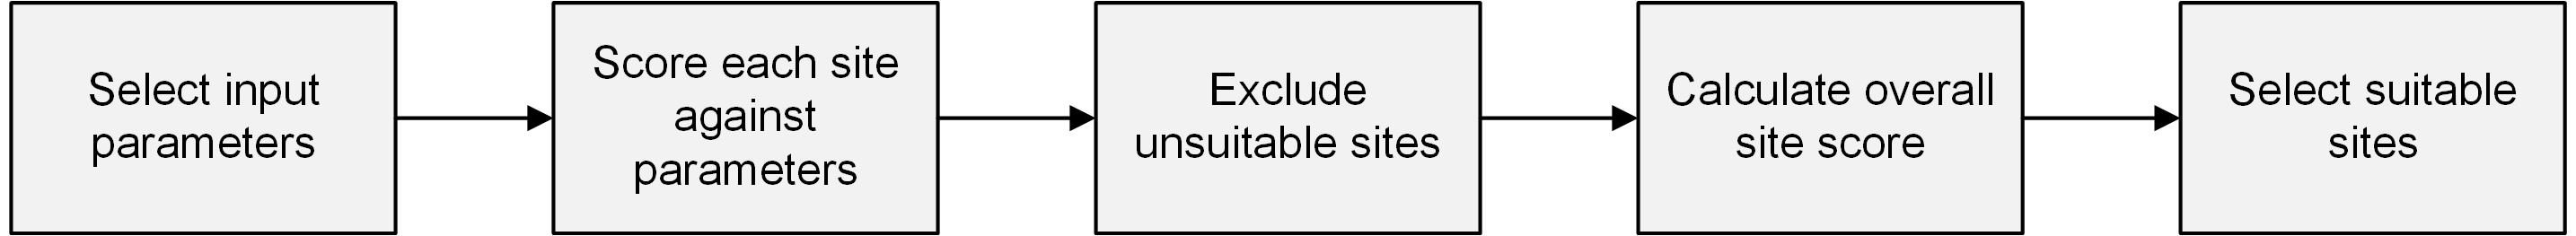
\includegraphics[width=1\linewidth]{figures/MethodologyFlowChart} \caption{An overview of the typical structure of GIS-MCDA methodologies}\label{fig:Flowchart}
\end{figure}

For remaining sites which could be developed, a score is calculated to
assess the overall suitability of the site. While several techniques are
used, the Weighted Sum Method (WSM) is most typically used as a method
to combine the different layers into a single score as follows:

\begin{equation}
 A_{i}^{WSM} = \sum_{j=1}^{n} w_{j} a_{ij} \quad \text{for} \quad i = 1,2,3,...N
  \label{eq:WSM}
\end{equation}

where \(w\) is the parameter weighting, \(a\) is the parameter value and
\(i\) is the attribute layer in the model. This rating can then be used
to determine the most suitable sites for development.

A concern surrounding the WSM is that the method is often applied
without any insight into the meanings of two critical elements: the
weights assigned to attribute layers and the procedures for combining
the layers (Malczewski \protect\hyperlink{ref-Malczewski2004}{2004}).
While methods such as the Analytic Hierarchy Procedure (AHP) are used to
mitigate this (Watson and Hudson, 2015), models remain highly sensitive
to the weightings used, and there are concerns that models result
provide the sub-optimal location of wind turbine locations, as
demonstrated by the high level of projects being refused planning
permission within the UK.

To address concerns of parameter weighting, there has been increased
interest in quantitatively assessing which parameters influence the
likelihood of wind turbines receiving planning permission (Rensburg,
Kelley, and Jeserich \protect\hyperlink{ref-VanRensburg20}{2015}). This
approach has recently been integrated within GIS modelling to assess the
influence of geospatial parameters in the UK (Harper et al.
\protect\hyperlink{ref-Harper2017}{2017}). This can be considered as a
form of retrospective GIS analysis, where the existing spatial
distribution of sites is assessed to enable prediction of where future
turbines may be acceptable. Harper et al's results suggest that the 1)
\emph{the number of wind turbines}; 2) \emph{percentage of the local
population with high levels of qualifications}; 3) \emph{the average
age} and 4) \emph{local political composition} emerge as key influences
affecting planning approval, while other typically used parameters such
as proximity to urban areas appear less influential. However, these
finding have yet to be integrated into a GIS-MCDA.

Finally, the issue of the standardisation of non-commensurate criteria
within the WSM and GIS-MCDA has yet to be satisfactorily addressed. To
create a single site suitability score requires the combination of a
range of economic, environmental and social parameters which cannot
directly be summed together into a single scale. Methods such as the
linear transformation method are often used to standardise each
variable, but there is limited empirical justification for such
approaches (Jiang and Eastman \protect\hyperlink{ref-Jiang2000}{2000}).

This paper addresses these concerns and presents the results of a
GIS-MCDA model that integrates planning acceptance rates into modelling.
This approach builds upon our previous work and demonstrates an
alternative layered approach combining non-commensurate parameters, in
particular avoiding the use of linear transformations within the MCDA.

\section{Methodology}\label{methodology}

The overall structure of the GIS model is shown in Figure
\ref{fig:Methodology}, and the stages are described in the following
subsections.

\begin{figure}[!h]
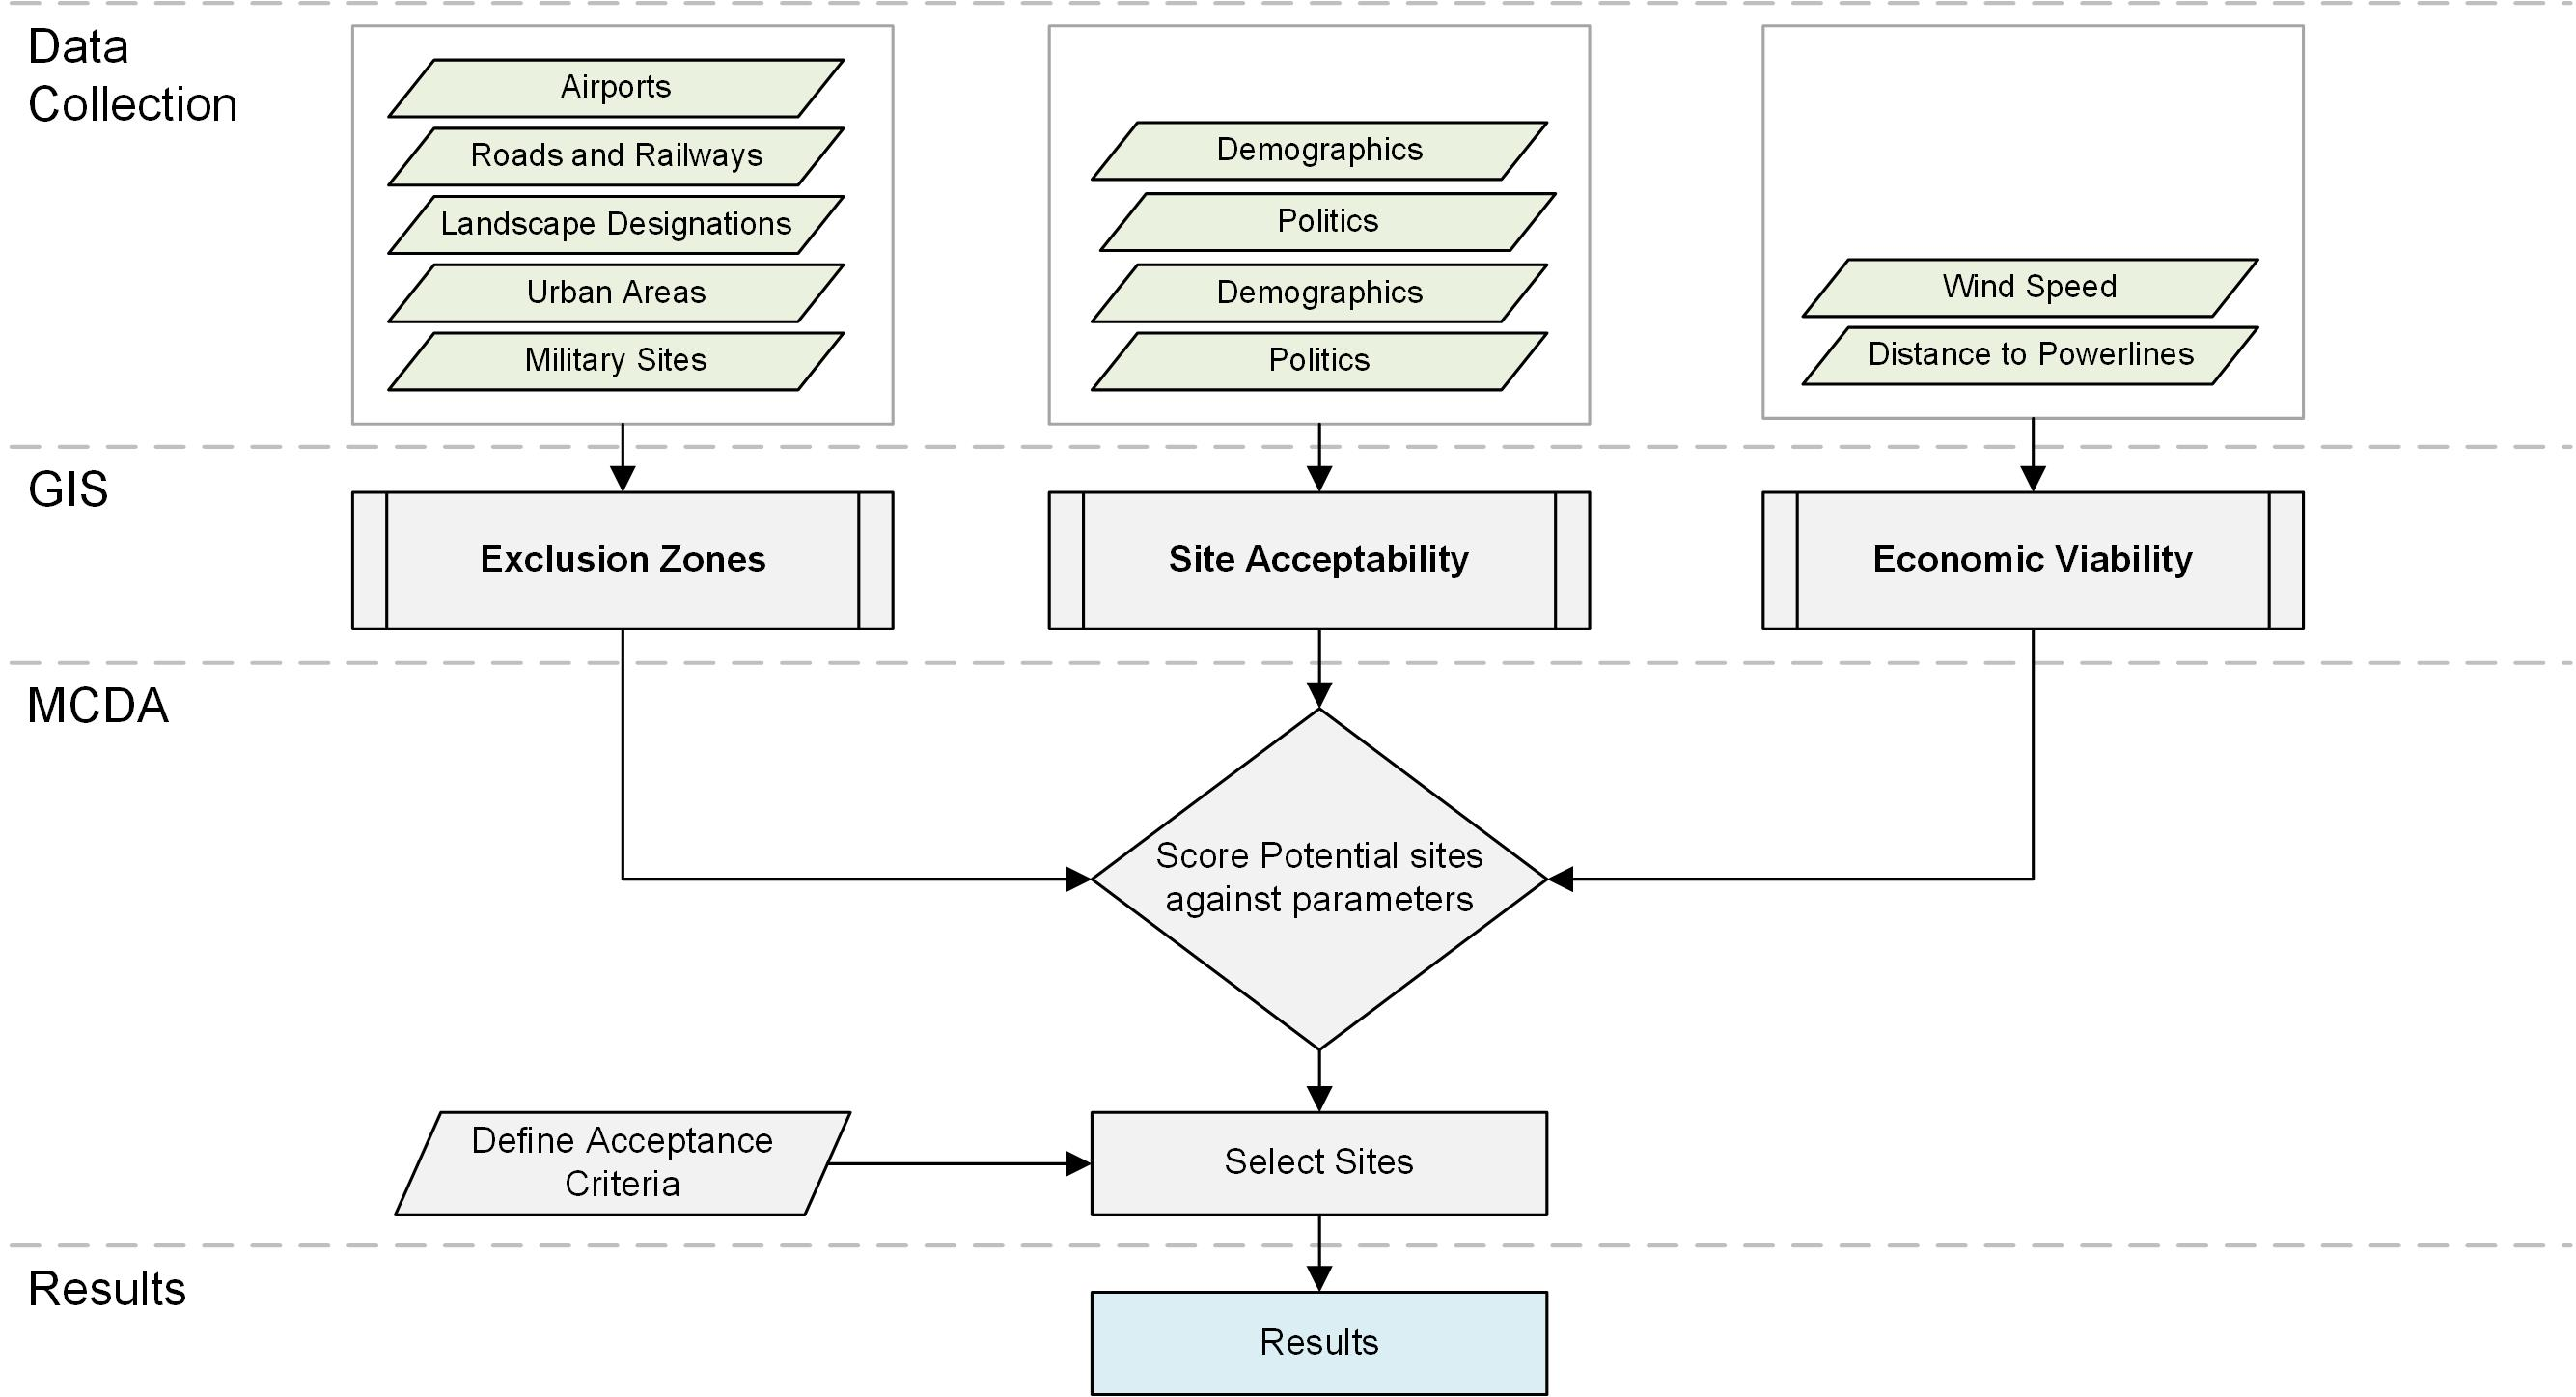
\includegraphics[width=1\linewidth]{figures/Flowchart for GIS Model} \caption{Overview of the onshore wind GIS-MCDA Structure}\label{fig:Methodology}
\end{figure}

\subsection{Model formation}\label{model-formation}

A preliminary scoping study was conducted to formulate the model and
identify parameters which influence wind turbine developments. The
identification of criteria involves a systematic analysis of factors
that may impact installation of the wind farms. This considered a range
of academic work as listed in Section 2, consultancy reports (Land Use
Consultants \protect\hyperlink{ref-LandUseConsultants2010}{2010}; SQW
Energy \protect\hyperlink{ref-SQWEnergy2010}{2010}) and wind turbine
planning guidance (Smith \protect\hyperlink{ref-Smith2016}{2016}).

The study was conducted across Great Britain (England, Scotland \&
Wales). This was chosen because of the broadly similar categorisation of
land types, nature designation, data availability and legislation across
these regions. To allow for a more detailed understanding of the local
effects, this paper also highlights the results from two case study
areas, Solent and the Midlands, as shown in Figure 3. These two areas
were selected as there are large differences in the number of wind
turbines deployed, with no wind turbines within the Solent region while
30 projects have been constructed within the Midlands region (DECC
\protect\hyperlink{ref-DECC2016}{2016}).

\begin{figure}[!h]
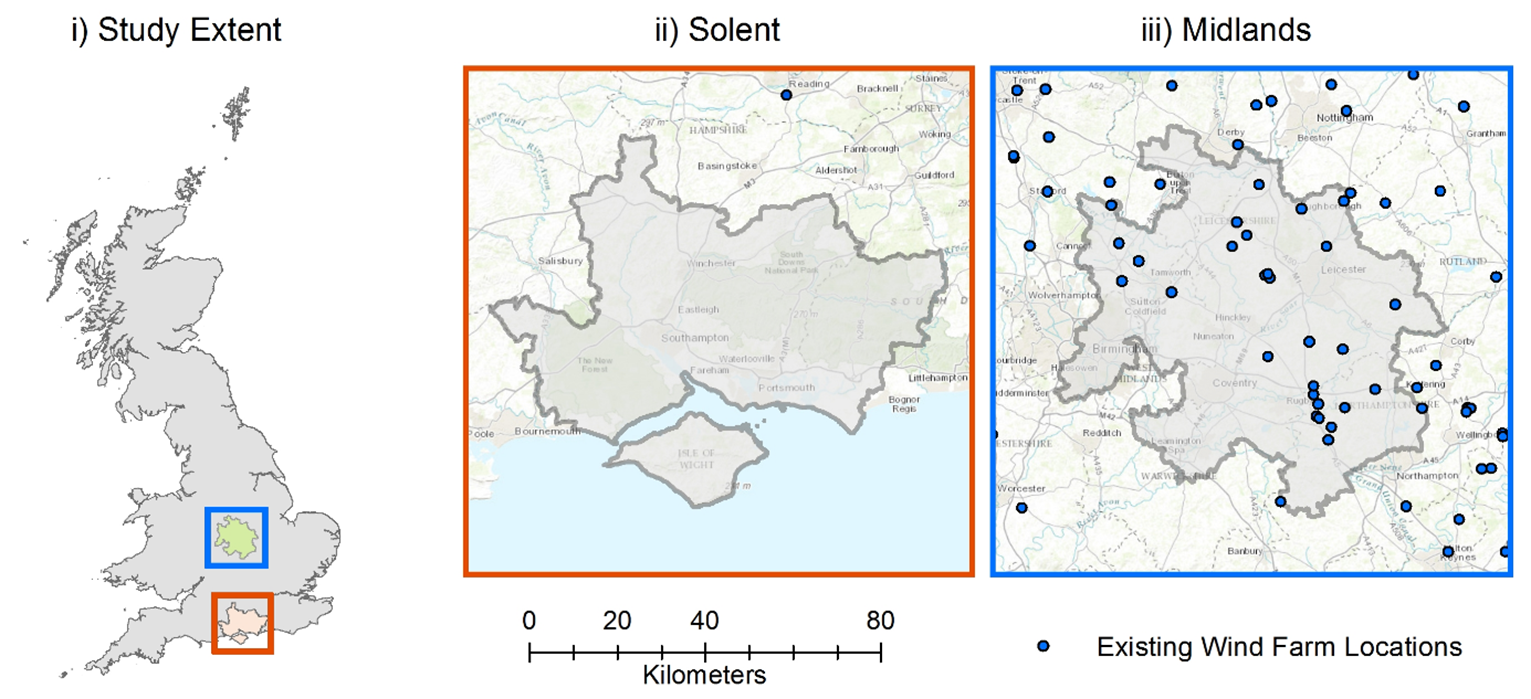
\includegraphics[width=1\linewidth]{figures/StudyExtent} \caption{Analysis Extent and regions selected for case studies, highlighting the locations of existing wind turbine projects}\label{fig:StudyExtent}
\end{figure}

Once key parameters were identified, relevant data was collected from a
range of sources for geospatial (OSM
\protect\hyperlink{ref-Overpass2016}{2016}; Ordnance Survey
\protect\hyperlink{ref-Survey2016}{2016}), environmental (SNH
\protect\hyperlink{ref-SNH2015}{2015}) and demographic variables (Office
for National Statistics
\protect\hyperlink{ref-OfficeforNationalStatistics}{2016}). A full
explanation of the datasets is available within the previous work
(Harper et al. \protect\hyperlink{ref-Harper2017}{2017}).

\subsection{GIS Model}\label{gis-model}

As highlighted within the background literature, there are challenges in
combining non-commensurate data within MCDA. Instead of combining
variables into a single score, an approach was developed to group input
variables into layers based on their type of influence on a site
suitability, with three layer GIS layers being formed; 1) \emph{Site
acceptability}; 2) \emph{Exclusion zones} and 3) \emph{Economic
viability}. These are explained in more detail as follows.

Site acceptability assess whether the chance of the location receiving
planning permission. This layer is based on previous analysis which used
logistic regression methods to identify the key influential parameters
that determine whether a wind turbine successfully obtained planning
consent (Harper et al., 2017). An overall predictive accuracy of 63\%
was achieved with the model, with the most influential parameters shown
in Table \ref{tab:TableofParameters}. The Odds Ratio shown indicates how
much the predicted planning acceptance rate changes for each unit of the
parameter. For example, for each km a site is further away from an urban
region, its likelihood of receiving planning approval increases by
0.176\%.

\begin{table}

\caption{\label{tab:TableofParameters}Parameters determined to influence the planning acceptance of wind turbines}
\centering
\begin{tabular}[t]{llrl}
\toprule
Parameter & Unit & Odds Ratio & Note\\
\midrule
Turbine Capacity & MW & 0.311 & Set as 2MW (a single turbine)\\
Urban Regions & km & 0.176 & Expressed as kilometre to each feature\\
AONB & km & 0.009 & \\
National Parks & km & 0.007 & \\
RAMSAR & km & -0.008 & \\
\addlinespace
SPA & km & -0.012 & \\
Qualification Perfect Level 4 & \% of Population & -0.031 & \\
Mean Age & years & -0.052 & \\
Time of Construction & years & -0.110 & Assumed to be 2017 within the model\\
\bottomrule
\end{tabular}
\end{table}

Exclusion Zones considers whether the site can be used for development.
Existing legislation and ecological guidance was reviewed, and the
geospatial development patterns of existing wind farms were assessed to
identify whether specific regions were avoided by developers. These
criteria were split into the following taxonomy:

\begin{itemize}
\tightlist
\item
  \textbf{Hard Planning Criteria}: these are legislative restrictions
  that prevent the development in specific areas. For example, wind
  turbines must not be built within a toppling distance of main roads.
\item
  \textbf{Soft Planning Criteria}: these are derived from statistical
  analysis of existing wind turbine planning applications to understand
  regions where turbines were generally not proposed but not
  legislatively restricted. For example, while it is technically
  possible to build in National Parks, only two projects have been built
  within them and therefore these regions can be considered as
  non-developable areas. This also excludes sites of ecological
  protection.
\item
  \textbf{Buffer Criteria}: explores whether there is any geospatial
  trend for sites to be located away from certain features. For example,
  wind turbines sites are not banned near airports, but sites are skewed
  away from these sites suggesting planners aim to keep distance between
  the sites. The values used within each of the exclusion layers are
  shown Table 2. Based on these three categories, three scenarios were
  formed to assess the impact of planning restrictions on the
  development potential: 1) \emph{Low Restriction} (Hard Planning
  Criteria only) 2) \emph{Medium Restriction} (Hard \& Soft Planning
  Criteria) and 3) \emph{High Restriction} (Hard, Soft and Buffer).
\end{itemize}

\begin{table}

\caption{\label{tab:unnamed-chunk-1}Parameters and exclusion distances used within the model}
\centering
\begin{tabular}[t]{llll}
\toprule
\multicolumn{1}{c}{ } & \multicolumn{3}{c}{Exclusion Distance, km} \\ \cmidrule(l{2pt}r{2pt}){2-4}
Parameter & Hard Planning Criteria & Soft Planning Criteria & Buffer Criteria\\
\midrule
Airports & 0 & 2.00 & 10.00\\
Roads & 0.15 & 0.15 & 0.15\\
Railways & 0.15 & 0.15 & 0.15\\
Military Sites & - & 0.00 & 10.00\\
Urban Areas & - & 0.00 & 2.00\\
\addlinespace
Powerlines & 0.15 & 0.15 & 0.15\\
Landscape Designations \textsuperscript{a} & - & 0.00 & 2.00\\
Nature Designations \textsuperscript{b} & - & 0.00 & 2.00\\
\bottomrule
\multicolumn{4}{l}{\textsuperscript{a} National Parks, Areas of Outstanding Natural Beauty, Heritage Coast}\\
\multicolumn{4}{l}{\textsuperscript{b} National Nature Reserves (NNR), Natura 2000, Special Protection Areas (SPA), Sites}\\
\multicolumn{4}{l}{of Special Scientific Interest (SSSI)}\\
\end{tabular}
\end{table}

Finally, economic suitability of the potential financial return of the
site. This layer was determined based on the wind speed and proximity of
the site to the distribution network. Potential wind power output was
calculated using the Weibull probability distribution combined with
logarithmic hub height correction.

Each of the layers were calculated as a raster layer, with a spatial
resolution of 250 metres, and were analysed and integrated using R and
supporting geospatial packages \emph{raster} (Hijmans
\protect\hyperlink{ref-raster}{2016}) and \emph{sp} (Roger S. Bivand,
Edzer Pebesma
\protect\hyperlink{ref-RogerS.BivandEdzerPebesma2013}{2013}).

\subsection{Multi-Criteria Decision
Analysis}\label{multi-criteria-decision-analysis}

The model considered the suitability of a site for the installation of
single wind turbines, and was based on a 2MW wind turbine which
represents the average size of onshore turbines constructed in 2016
(Vestas \protect\hyperlink{ref-Vesta2017}{2017}). Based on planning
guidance, a spacing between turbines of 500m was used (Smith
\protect\hyperlink{ref-Smith2016}{2016}), resulting in a development
density of 8MW/km\textsuperscript{2}.

As shown in Figure 4, each site is categorised based on its Economic
viability (X-axis) and Site Suitability (Y-axis), with four types of
suitability defined (Low/Potential/Good/Excellent). More flexibility is
given to the site suitability parameter to reflect that there is less
certainty to this value. The analysis selected sites based on their
suitability rating. To estimate the potential capacity of sites that
could be developed, all sites that score ``\emph{Excellent}'' or
``\emph{Good}'' were selected as suitable for development.

\begin{figure}[!h]
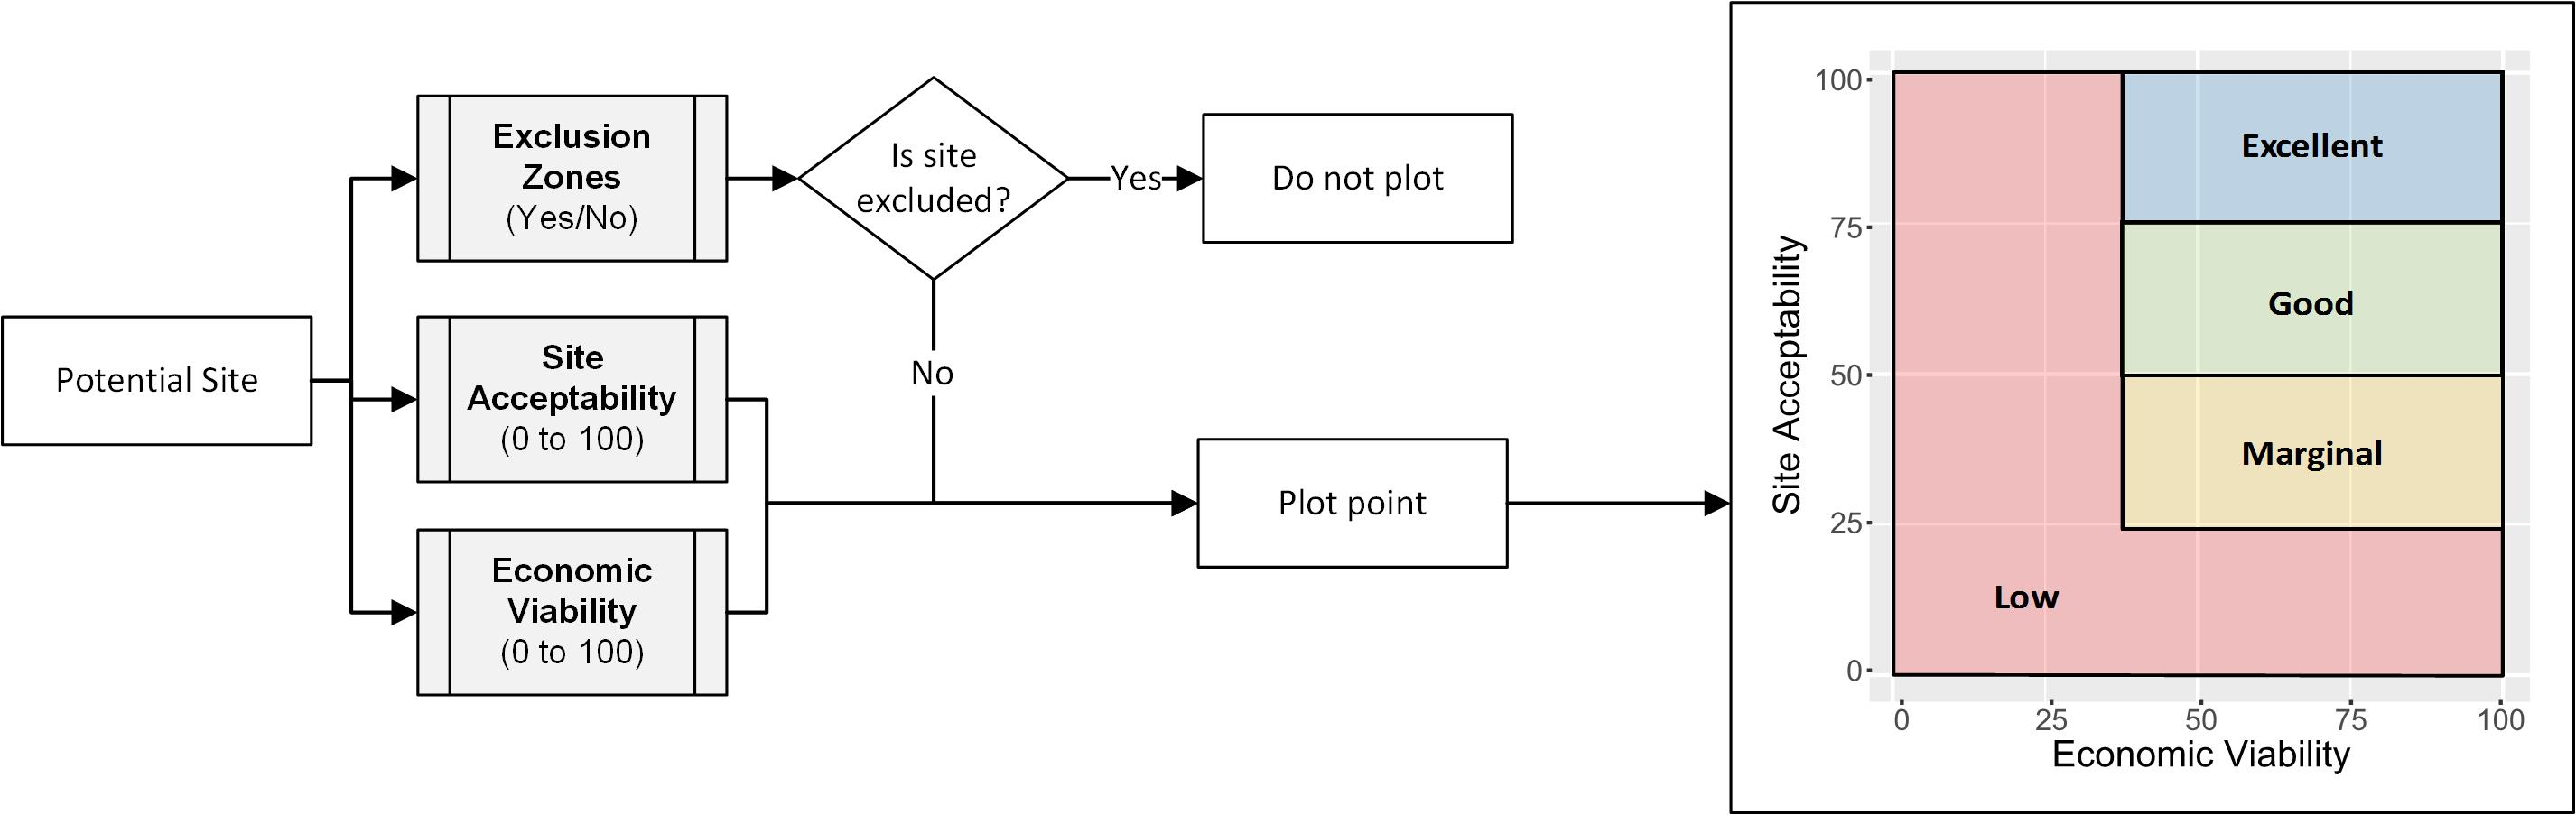
\includegraphics[width=1\linewidth]{figures/GIS Plot V2} \caption{Classification of potential sites based on the GIS layer results}\label{fig:SiteProcess}
\end{figure}

\section{Results}\label{results}

The results from the geospatial model layers are presented in Figure
\ref{fig:GISLayers}, which shows the three separate layers of the
analysis. These layers are combined to determine the site suitability
score displayed under the medium development restriction scenario, as
shown Figure 6. Nationally, it can be seen from the results that sites
appear to be more suitable within Scotland, the South East of England,
and patches of West England. For the Solent region, 77\% of the land was
excluded with no sites being deemed ``Good'' or ``Excellent'' for wind
development. In comparison, 45\% of the Midlands region was excluded for
development with 1.2GW of potential site capacity identified from
suitable sites.

\begin{figure}[!h]
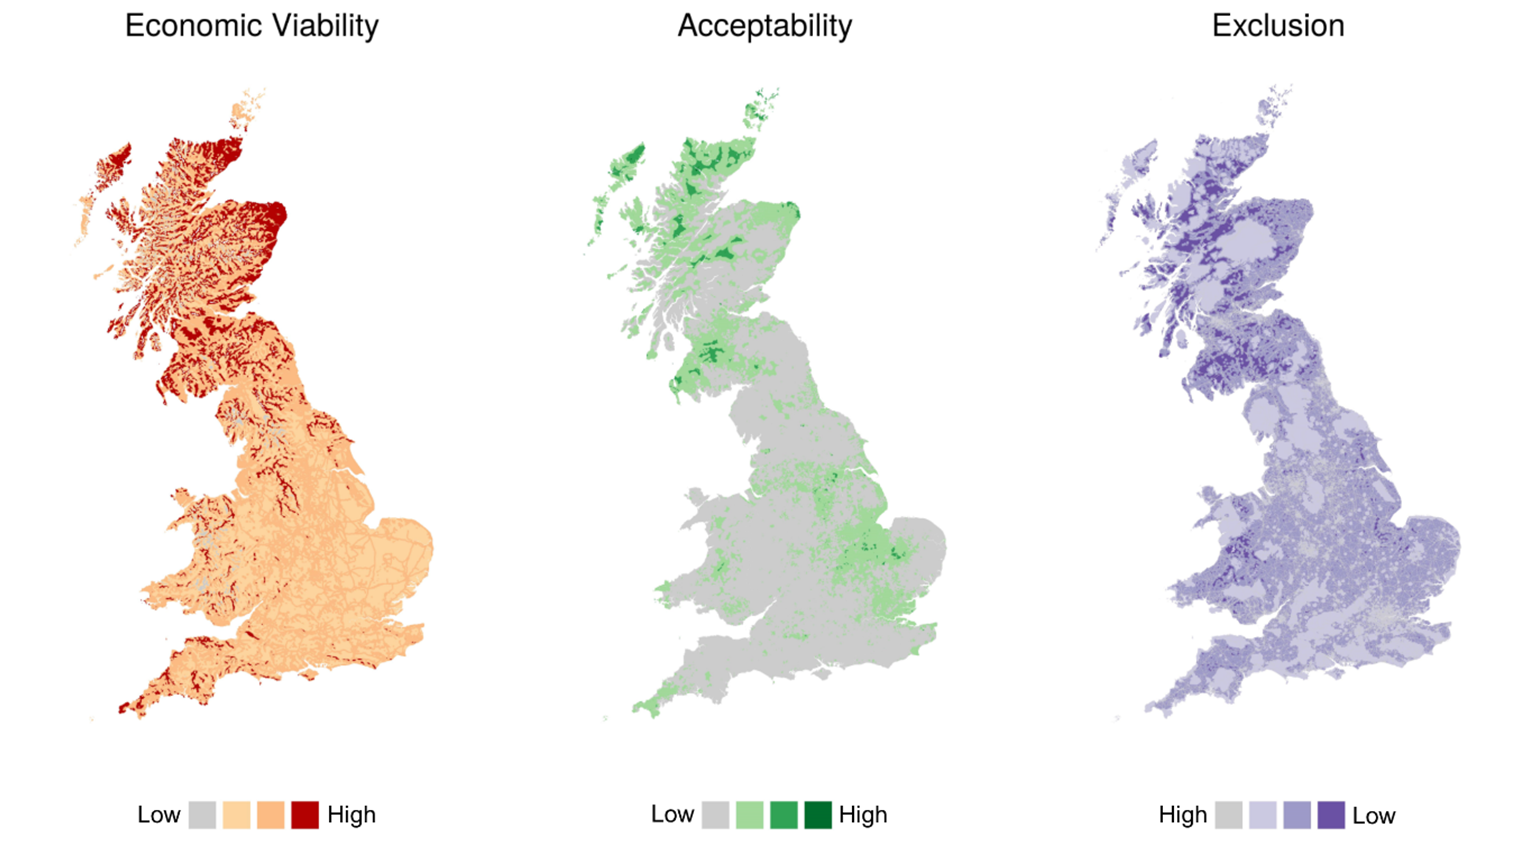
\includegraphics[width=1\linewidth]{figures/GISLayers} \caption{Results for the three onshore wind GIS layers within the model. Darker colours indicate desirable characteristics for wind turbine sites}\label{fig:GISLayers}
\end{figure}

\begin{figure}[!h]
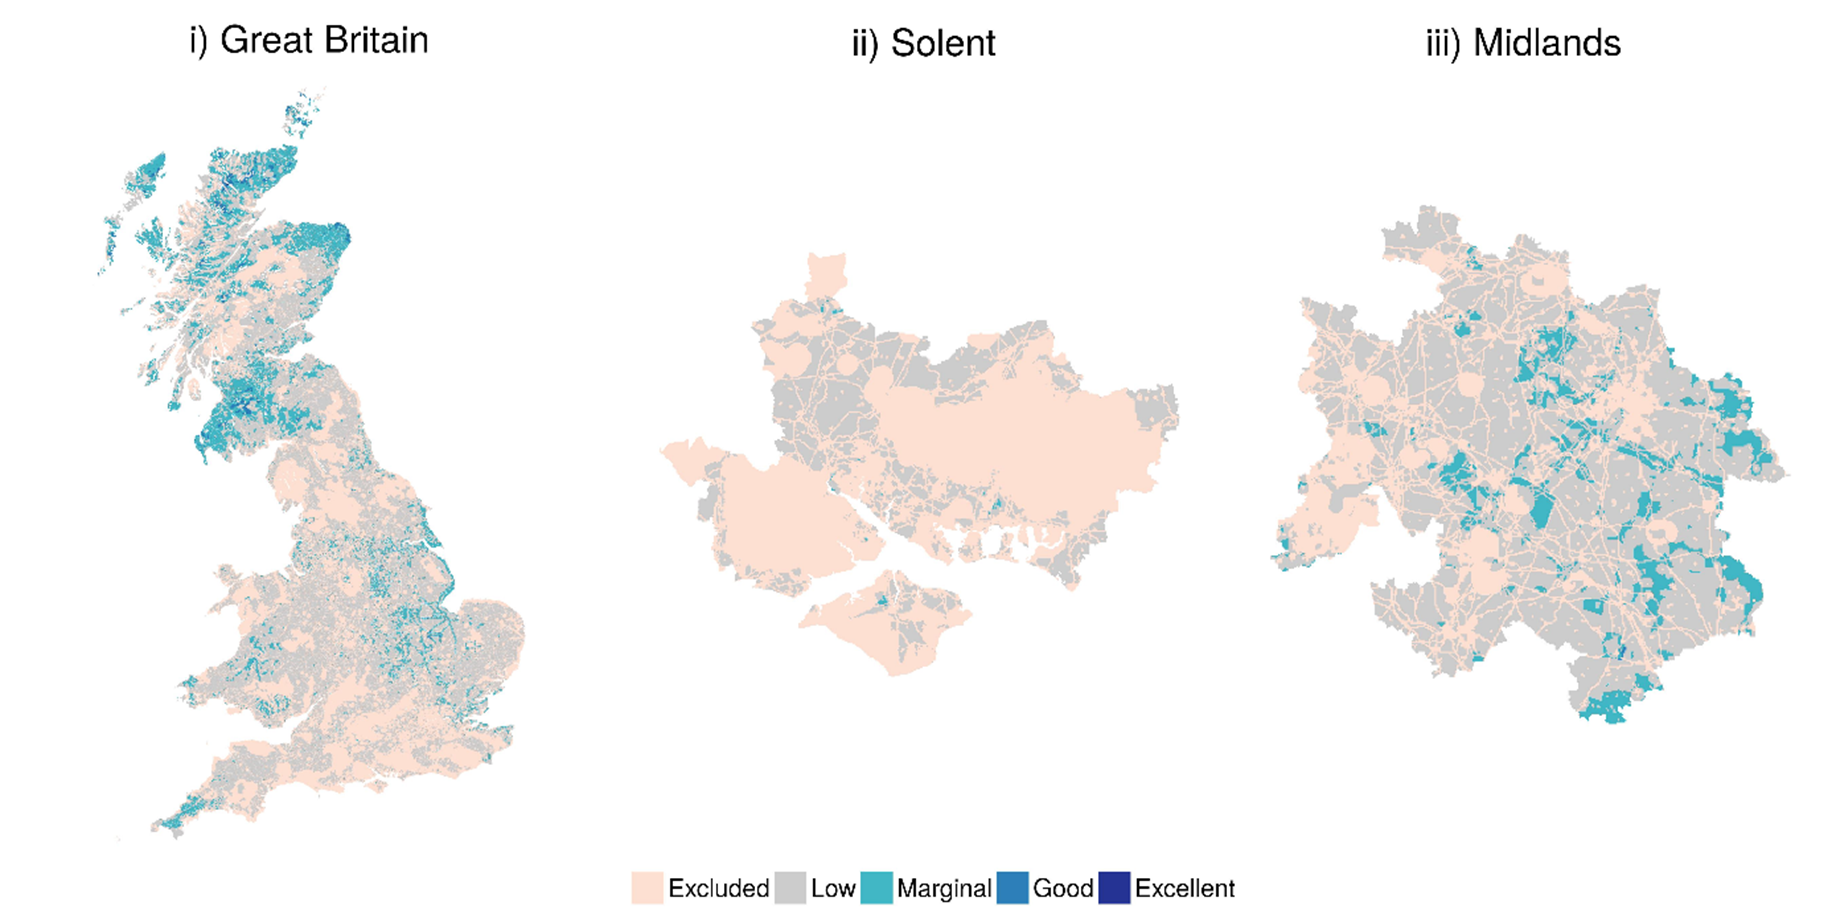
\includegraphics[width=1\linewidth]{figures/ResultsMap} \caption{Comparison of Wind Turbine Potential under the medium development scenario}\label{fig:ResultsMap}
\end{figure}

Table \ref{tab:ScoreMatrix} provides a detailed breakdown of the land
suitability under of the each of the three exclusion regions for the
national model. Cells highlighted in grey indicate those which are the
most suitable for development potential, being outside crucial exclusion
zones and having a high site suitability score. Such sites cover 0.74\%
of the country, and represents 13GW of potential capacity if fully
utilised.

\begin{table}

\caption{\label{tab:ScoreMatrix}Site score suitability matrix comparing exclusion criteria against site suitability, coverage of land covered by each classification}
\centering
\begin{tabular}[t]{lrrrrr}
\toprule
Suitability Score & Hard Criteria & Soft Criteria & Buffer Criteria & No Exclusion & Total\\
\midrule
Low & 11.430 & 25.580 & 37.700 & 2.82 & 77.500\\
Marginal & 2.780 & 5.900 & 8.980 & 3.07 & 20.720\\
Good & 0.070 & 0.930 & 0.510 & 0.23 & 1.740\\
Excellent & 0.000 & 0.005 & 0.003 & 0.00 & 0.008\\
Total & 14.275 & 32.418 & 47.186 & 6.12 & 100.000\\
\bottomrule
\end{tabular}
\end{table}

The comparative suitability of the regions can also be explored through
density plots as shown in Figure \ref{fig:DensityPlot}. Each
non-excluded site is represented as a point, and the regional variation
in acceptability and economic viability can be viewed on separate
scales. The site acceptability within the Solent region is generally
less than the national average and the Midlands, although the economic
viability is generally similar.

\begin{figure}[!h]
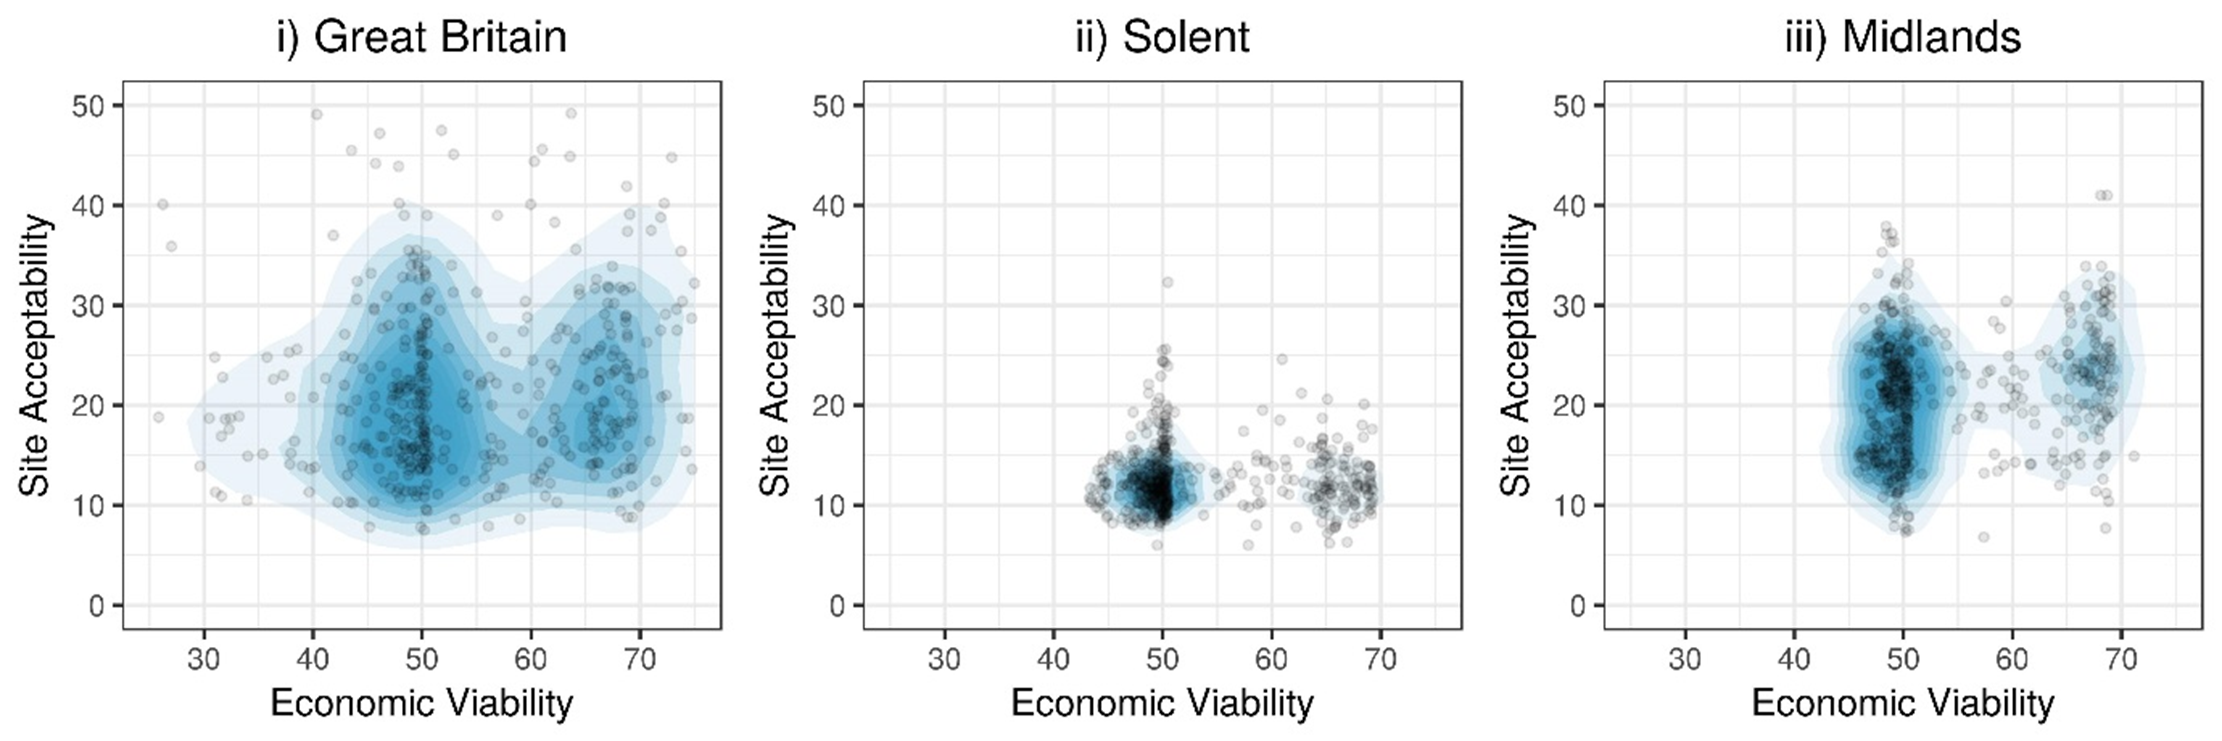
\includegraphics[width=1\linewidth]{figures/DensityPlots} \caption{Two-dimensional Density Plots for wind turbine sites within the the Midlands and Hampshire/Solent regions. Note that the axes have been truncated at a score of 50}\label{fig:DensityPlot}
\end{figure}

\section{Discussion}\label{discussion}

The analysis suggests that 13GW of onshore wind would be highly suitable
within a medium development restriction scenario, which considered the
``hard'' and ``soft'' planning criteria. If the stricter ``buffer''
criteria are met, the estimated capacity is reduced to 4 GW. Both these
estimates are significantly lower than previous studies which have
suggested total capacity could exceed 200 GW (Stoddart and Turley, 2012;
Gove et al., 2016). This highlights the impact of considering likelihood
of planning acceptance within the GIS-MCDA and the constraint this
places on development.

The case studies of Solent and Midlands highlight the regional
variations in onshore wind potential resource as shown in Figures 6 and
7. From a resource perspective, the Solent area is highly suitable with
many hilly regions and its coastal location resulting in high wind
speeds. However, the opportunity for development is limited by National
Parks and Areas of Outstanding Natural Beauty (AONB), and the sites that
are located outside of these regions are largely unsuitable for
development due to the demographic composition. In comparison, the the
Midlands region faces much less restriction in where developments could
be made and presents much greater opportunity for future development.

The results further highlight that cost is not the dominant issue in
determining the suitability of a wind turbine site, as wind speeds are
largely satisfactory and in UK most sites are an acceptance distance to
powerlines for a wind turbine to be economic. A number of previous
studies have placed a high weighting on wind resource (Shirgholami,
Namdar Zangeneh, and Bortolini
\protect\hyperlink{ref-Shirgholami2016}{2016}), reflecting the interest
of the developer to maximise returns. In reality, it may be in their
interest to select a less windy site that is more likely to receive
planning permission.

On a national level, it is important to consider the distribution of
potential sites and the consequent impact this may have on the
electricity transmission network. The results indicate that regions in
Scotland and the South West are most suitable for further development;
however, such areas are distant to large load centres such as cities,
requiring transmission networks or energy storage to be upgraded.

A benefit of building the model into several intermediate layers, such
as used in this model, is that it allows the results to be more easily
interpreted and minimise the concerns surrounding standardisation of
parameters. When combining the variables into a single suitability
score, it can easily hide or distort what is influencing the site score,
and make it difficult to understand why some sites are more suitable
than others are.

\section{Limitations \& Future Work}\label{limitations-future-work}

Such models are highly influenced by the availability and quality of the
data¬ for the analysis. Wind speed is only available at 1km resolution
and does not account for roughness of surface caused by urban
developments of varying land cover such as forests (DTI
\protect\hyperlink{ref-DTI2001}{2001}). The errors from any dataset will
have propagated through the analysis and, combined with errors from
other layers, may cause inaccuracies in the output map. Future work will
therefore investigate the sensitivity of results.

Whilst the analysis has tried to understand the chance of a project
being accepted, it has only considered geospatial parameters. As
previous studies have highlighted, such parameters in themselves only
provide part of the explanation as to why wind farms are accepted
(Langer et al. \protect\hyperlink{ref-Langer2016a}{2016}; Dave Toke
\protect\hyperlink{ref-Toke2005}{2005}). Greater emphasis must also be
placed on the planning process and local engagement of a wind project if
it is to be successful at planning.

The analysis has also not considered the impact of electricity
transmission networks, and the potential requirement of grid
reinforcements. It is already being seen in the UK that grid
reinforcements are being made to transfer electricity and this is
becoming a limiting factor in the development of renewable energy
projects (National Grid \protect\hyperlink{ref-NationalGrid2015}{2015}).
The majority of sites identified as suitable for development are distant
from large load centres, and therefore would place additional strain on
the transmission network to transfer this electricity across the
country. It is therefore important that this issue is explored further
in future analysis.

The model only considers the suitability of individual wind turbines,
and does not assess whether an area is suitable for development of a
larger wind farm. There would be economies of scale in proposing a
single larger development, and as such, these locations would be
preferential to developers.

The analysis did not consider the influence of the cumulative number of
wind turbines within a certain area. It is not fully understood within
literature whether there is a limit to the development potential of wind
turbines, although some evidence suggests that regions can reach a
saturation level (David Toke, Breukers, and Wolsink
\protect\hyperlink{ref-Toke2008}{2008}).

\section{Conclusion}\label{conclusion}

The authors' have presented a GIS-MCDA which can be used to assist in
location onshore wind turbines. By integrating planning acceptance rates
into the decision-making process, the results of this model have
highlighted that the potential resource is significantly lower than
previous estimates. However, there remains an opportunity for further
development of onshore wind turbines to help meet renewable electricity
generation targets.

The GIS-MCDA presented an alternative method of combining
non-commensurate data into the decision-making process. By avoiding the
use of standardisation, there is less distortion to the input data and
this reduces potential errors within the model results. This also
provides greater insight into the model results as it is easier to
understand the factors influencing site suitability.

Using two case studies, the results have shown how the onshore wind
capacity can vary significantly for similar types of regions within the
same country. This can be influenced by physical restrictions such as
landscape and nature designations, or ``hidden'' factors such as local
demographics and political composition. It is therefore important that
these factors are understood when wind turbines are being considered
within a region.

The findings of this study can be used by a range of stakeholder to
improve the planning and development of wind turbines. As examples,
regional planners could more accurately estimate the potential capacity
within their region, and project developers could gain a greater
understanding of where sites should be proposed to increase the
likelihood of receiving planning permission. The results should support,
not replace, local level planning.

Whilst the analysis was completed within Great Britain, the concepts
developed can be applied internationally. However, the specific planning
acceptability data will have to be the region as outlined in previous
analysis (Harper et al. \protect\hyperlink{ref-Harper2017}{2017}).

\section*{Acknowledgements}\label{acknowledgements}
\addcontentsline{toc}{section}{Acknowledgements}

This work is part of the activities of the Energy and Climate Change
Division and the Sustainable Energy Research Group at the University of
Southampton \url{www.energy.soton.ac.uk}. It is also had financial
support from EPSRC grants: EP/J017698/1, Transforming the Engineering of
Cities to Deliver Societal and Planetary Wellbeing, EP/N010779/1,
City-Wide Analysis to Propel Cities towards Resource Efficiency and
Better Wellbeing and EP/K012347/1, International Centre for
Infrastructure Futures (ICIF).

\section*{References}\label{references}
\addcontentsline{toc}{section}{References}

\hypertarget{refs}{}
\hypertarget{ref-Atici2015}{}
Atici, Kazim Baris, Ahmet Bahadir Simsek, Aydin Ulucan, and Mustafa Umur
Tosun. 2015. ``A GIS-based Multiple Criteria Decision Analysis approach
for wind power plant site selection.'' \emph{Utilities Policy} 37.
Elsevier Ltd: 86--96.
doi:\href{https://doi.org/10.1016/j.jup.2015.06.001}{10.1016/j.jup.2015.06.001}.

\hypertarget{ref-Baban2001}{}
Baban, Serwan M J, and Tim Parry. 2001. ``Developing and applying a
GIS-assisted approach to locating wind farms in the UK.''
\emph{Renewable Energy} 24 (1): 59--71.
doi:\href{https://doi.org/10.1016/S0960-1481(00)00169-5}{10.1016/S0960-1481(00)00169-5}.

\hypertarget{ref-DECC2016}{}
DECC. 2016. ``Renewable Energy Planing Data.''
\url{https://www.gov.uk/government/collections/renewable-energy-planning-data}.

\hypertarget{ref-DTI2001}{}
DTI. 2001. ``NOABL Windspeed Database.'' \url{https://goo.gl/6BALyv}.

\hypertarget{ref-Gigovic2017}{}
Gigović, Ljubomir, Dragan Pamučar, Darko Božanić, and Srđan Ljubojević.
2017. ``Application of the GIS-DANP-MABAC multi-criteria model for
selecting the location of wind farms: A case study of Vojvodina,
Serbia.'' \emph{Renewable Energy} 103: 501--21.
doi:\href{https://doi.org/10.1016/j.renene.2016.11.057}{10.1016/j.renene.2016.11.057}.

\hypertarget{ref-Gove2016a}{}
Gove, Benedict, Leah J. Williams, Alison E. Beresford, Philippa Roddis,
Colin Campbell, Emma Teuten, Rowena H W Langston, and Richard B.
Bradbury. 2016. ``Reconciling biodiversity conservation and widespread
deployment of renewable energy technologies in the UK.'' \emph{PLoS ONE}
11 (5): 1--30.
doi:\href{https://doi.org/10.1371/journal.pone.0150956}{10.1371/journal.pone.0150956}.

\hypertarget{ref-Harper2017}{}
Harper, Michael, Ben Anderson, Patrick James, and a. S. Bahaj. 2017.
``Identifying key influences for planning acceptance of onshore wind
turbines.'' In \emph{Proceedings of Ecos 2017 - the 30th International
Conference on Efficiency, Cost, Optimization, Simulation and
Environmental Impact of Energy Systems}.

\hypertarget{ref-raster}{}
Hijmans, Robert J. 2016. ``raster: Geographic Data Analysis and
Modeling.'' \url{https://cran.r-project.org/package=raster}.

\hypertarget{ref-Janke2010}{}
Janke, J. R. 2010. ``Multicriteria GIS modeling of wind and solar farms
in Colorado.'' \emph{Renewable Energy} 35: 2228--34.
\href{http://people.umass.edu/bethanyb/Janke,\%202010.pdf}{http://people.umass.edu/bethanyb/Janke, 2010.pdf}.

\hypertarget{ref-Jiang2000}{}
Jiang, Hong, and J. Ronald Eastman. 2000. ``Application of fuzzy
measures in multi-criteria evaluation in GIS.'' \emph{International
Journal of Geographical Information Science} 14 (2): 173--84.
doi:\href{https://doi.org/10.1080/136588100240903}{10.1080/136588100240903}.

\hypertarget{ref-LandUseConsultants2010}{}
Land Use Consultants. 2010. ``Review of Renewable and Decentralised
Energy Potential in South East England ( June 2010 ).'' \emph{East}, no.
June.

\hypertarget{ref-Langer2016a}{}
Langer, Katharina, Thomas Decker, Jutta Roosen, and Klaus Menrad. 2016.
``A qualitative analysis to understand the acceptance of wind energy in
Bavaria.'' \emph{Renewable and Sustainable Energy Reviews} 64. Elsevier:
248--59.
doi:\href{https://doi.org/10.1016/j.rser.2016.05.084}{10.1016/j.rser.2016.05.084}.

\hypertarget{ref-Malczewski2004}{}
Malczewski, Jacek. 2004. ``GIS-based land-use suitability analysis: A
critical overview.'' \emph{Progress in Planning} 62 (1): 3--65.
doi:\href{https://doi.org/10.1016/j.progress.2003.09.002}{10.1016/j.progress.2003.09.002}.

\hypertarget{ref-Miller2014}{}
Miller, Adam, and Ruopu Li. 2014. ``A Geospatial Approach for
Prioritizing Wind Farm Development in Northeast Nebraska, USA.''
\emph{ISPRS International Journal of Geo-Information} 3 (3): 968--79.
doi:\href{https://doi.org/10.3390/ijgi3030968}{10.3390/ijgi3030968}.

\hypertarget{ref-NationalGrid2015}{}
National Grid. 2015. ``Electricity Ten Year Statement 2015,'' no.
November: 136.

\hypertarget{ref-Neufville2013}{}
Neufville, Laurence. 2013. ``Wind farm Site Suitability Selection using
Multi-Criteria Analysis (MCA) and Spatial Modelling,'' no. July: 1--29.

\hypertarget{ref-Noorollahi2015}{}
Noorollahi, Younes, Hossein Yousefi, and Mohammad Mohammadi. 2015.
``Multi-criteria decision support system for wind farm site selection
using GIS.'' \emph{Sustainable Energy Technologies and Assessments} 13.
Elsevier Ltd: 38--50.
doi:\href{https://doi.org/10.1016/j.seta.2015.11.007}{10.1016/j.seta.2015.11.007}.

\hypertarget{ref-OfficeforNationalStatistics}{}
Office for National Statistics. 2016. ``2011 Census data.''
\url{https://www.ons.gov.uk/census/2011census/2011censusdata}.

\hypertarget{ref-Survey2016}{}
Ordnance Survey. 2016. ``OS Strategi.''
\url{https://data.gov.uk/dataset/strategi}.

\hypertarget{ref-Overpass2016}{}
OSM. 2016. ``Overpass API.'' \url{https://overpass-turbo.eu/}.

\hypertarget{ref-VanRensburg20}{}
Rensburg, Thomas M. van, Hugh Kelley, and Nadine Jeserich. 2015. ``What
influences the probability of wind farm planning approval: Evidence from
Ireland.'' \emph{Ecological Economics} 111. Elsevier B.V.: 12--22.
doi:\href{https://doi.org/10.1016/j.ecolecon.2014.12.012}{10.1016/j.ecolecon.2014.12.012}.

\hypertarget{ref-RogerS.BivandEdzerPebesma2013}{}
Roger S. Bivand, Edzer Pebesma, Virgilio Gomez-Rubio. 2013.
\emph{Applied spatial data analysis with R}. Second Edi. NY: Springer.

\hypertarget{ref-Shirgholami2016}{}
Shirgholami, Zahra, Soudabeh Namdar Zangeneh, and Marco Bortolini. 2016.
``Decision system to support the practitioners in the wind farm design:
A case study for Iran mainland.'' \emph{Sustainable Energy Technologies
and Assessments} 16. Elsevier Ltd: 1--10.
doi:\href{https://doi.org/10.1016/j.seta.2016.04.004}{10.1016/j.seta.2016.04.004}.

\hypertarget{ref-Sliz-Szkliniarz2011}{}
Sliz-Szkliniarz, Beata, and Joachim Vogt. 2011. ``GIS-based approach for
the evaluation of wind energy potential: A case study for the
Kujawsko-Pomorskie Voivodeship.'' \emph{Renewable and Sustainable Energy
Reviews} 15 (3). Elsevier Ltd: 1696--1707.
doi:\href{https://doi.org/10.1016/j.rser.2010.11.045}{10.1016/j.rser.2010.11.045}.

\hypertarget{ref-Smith2016}{}
Smith, Louise. 2016. ``Planning for onshore wind farms.'' \emph{House of
Commons Briefing Paper}, no. 04370.
\url{http://www.parliament.uk/briefing-papers/sn04370.pdf}.

\hypertarget{ref-SNH2015}{}
SNH. 2015. ``Sites of Specific Scientific Interest, Scotland.''
\url{https://gateway.snh.gov.uk/natural-spaces/index.jsp}.

\hypertarget{ref-SQWEnergy2010}{}
SQW Energy. 2010. ``Renewable and Low-carbon Energy Capacity Methodology
Methodology for the English Regions.'' January.

\hypertarget{ref-Toke2005}{}
Toke, Dave. 2005. ``Explaining wind power planning outcomes: Some
findings from a study in England and Wales.'' \emph{Energy Policy} 33
(12): 1527--39.
doi:\href{https://doi.org/10.1016/j.enpol.2004.01.009}{10.1016/j.enpol.2004.01.009}.

\hypertarget{ref-Toke2008}{}
Toke, David, Sylvia Breukers, and Maarten Wolsink. 2008. ``Wind power
deployment outcomes: How can we account for the differences?''
\emph{Renewable and Sustainable Energy Reviews} 12 (4): 1129--47.
doi:\href{https://doi.org/10.1016/j.rser.2006.10.021}{10.1016/j.rser.2006.10.021}.

\hypertarget{ref-VanHaaren2011}{}
Van Haaren, Rob, and Vasilis Fthenakis. 2011. ``GIS-based wind farm site
selection using spatial multi-criteria analysis (SMCA): Evaluating the
case for New York State.'' \emph{Renewable and Sustainable Energy
Reviews} 15 (7). Elsevier Ltd: 3332--40.
doi:\href{https://doi.org/10.1016/j.rser.2011.04.010}{10.1016/j.rser.2011.04.010}.

\hypertarget{ref-Vesta2017}{}
Vestas. 2017. ``2MW Turbine Specification.''
\url{http://nozebra.ipapercms.dk/Vestas/Communication/Productbrochure/2MWbrochure/2MWProductBrochure/}.

\hypertarget{ref-Voivontas1998}{}
Voivontas, D., D. Assimacopoulos, a. Mourelatos, and J. Corominas. 1998.
``Evaluation of renewable energy potential using a GIS decision support
system.'' \emph{Renewable Energy} 13 (3): 333--44.
doi:\href{https://doi.org/10.1016/S0960-1481(98)00006-8}{10.1016/S0960-1481(98)00006-8}.

\hypertarget{ref-Wang2014}{}
Wang, Qianna, Martin Mwirigi M'Ikiugu, and Isami Kinoshita. 2014. ``A
GIS-based approach in support of spatial planning for renewable energy:
A case study of Fukushima, Japan.'' \emph{Sustainability (Switzerland)}
6 (4): 2087--2117.
doi:\href{https://doi.org/10.3390/su6042087}{10.3390/su6042087}.

\hypertarget{ref-Watson2015}{}
Watson, Joss J W, and Malcolm D. Hudson. 2015. ``Regional Scale wind
farm and solar farm suitability assessment using GIS-assisted
multi-criteria evaluation.'' \emph{Landscape and Urban Planning} 138.
Elsevier B.V.: 20--31.
doi:\href{https://doi.org/10.1016/j.landurbplan.2015.02.001}{10.1016/j.landurbplan.2015.02.001}.


\end{document}
